\chapter{Introduction}

\paragraph*{}
This report aims to highlight the progress of our final project, \textbf{Collective Transport using Swarm Robotics}, with the evaluating criteria being the team individual contributions, as well as our pace in comparison to the ideal schedule. The ideal schedule can be represented by the project Gantt Chart (Figure \ref{fig:gantt_chart}).

\paragraph*{}
According to Figure \ref{fig:gantt_chart}, we are exploring four major sub-tasks during this iteration of the project schedule. These four tasks are: \textbf{Communication in the Swarm} (Task 1.1), \textbf{Simple Simultaneous Localization and Mapping (SLAM) in Simulation} (Task 1.2), \textbf{Coordinated Gripping and Formation} (Task 1.3), and \textbf{Object detection} (Task 1.4). These tasks are planned to span from January to the second week of March. The results of the endeavours will be discussed in the following chapters

\begin{figure}[H]
    \centering
    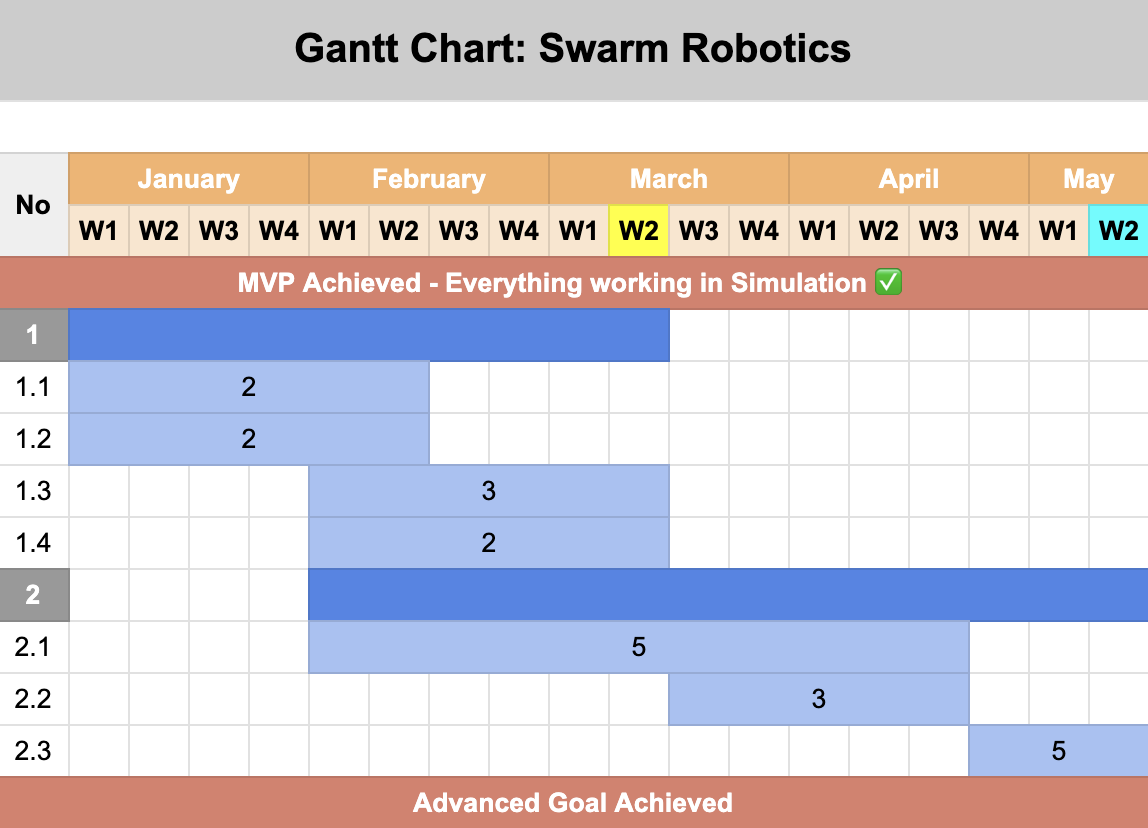
\includegraphics[width=1\linewidth]{assets/images/timeline/gantt_chart.png}
    \caption{Project Gantt Chart}
    \label{fig:gantt_chart}
\end{figure}

\begin{enumerate}
    \item Preparation for Hardware Implementation
    \begin{enumerate}[label=1.\arabic*]
        \item Communication in the swarm
        \item Simple Simultaneous Localization and Mapping (SLAM) in Simulation
        \item Coordinated Gripping and Formation
        \item Object detection
    \end{enumerate}
    \item Moving Towards a Complete Swarm
    \begin{enumerate}[label=2.\arabic*]
        \item Hardware
        \item Movement after Gripping
        \item Testing and Evaluation
    \end{enumerate}
\end{enumerate}
